\documentclass[border=10pt]{standalone}
\usepackage[svgnames]{xcolor}
\usepackage{amsmath}
\usepackage{pgfplots}
\pgfplotsset{compat=newest}
\usepackage[sfdefault]{FiraSans}
\usepackage{FiraMono}
\renewcommand*\familydefault{\sfdefault}
\begin{document}
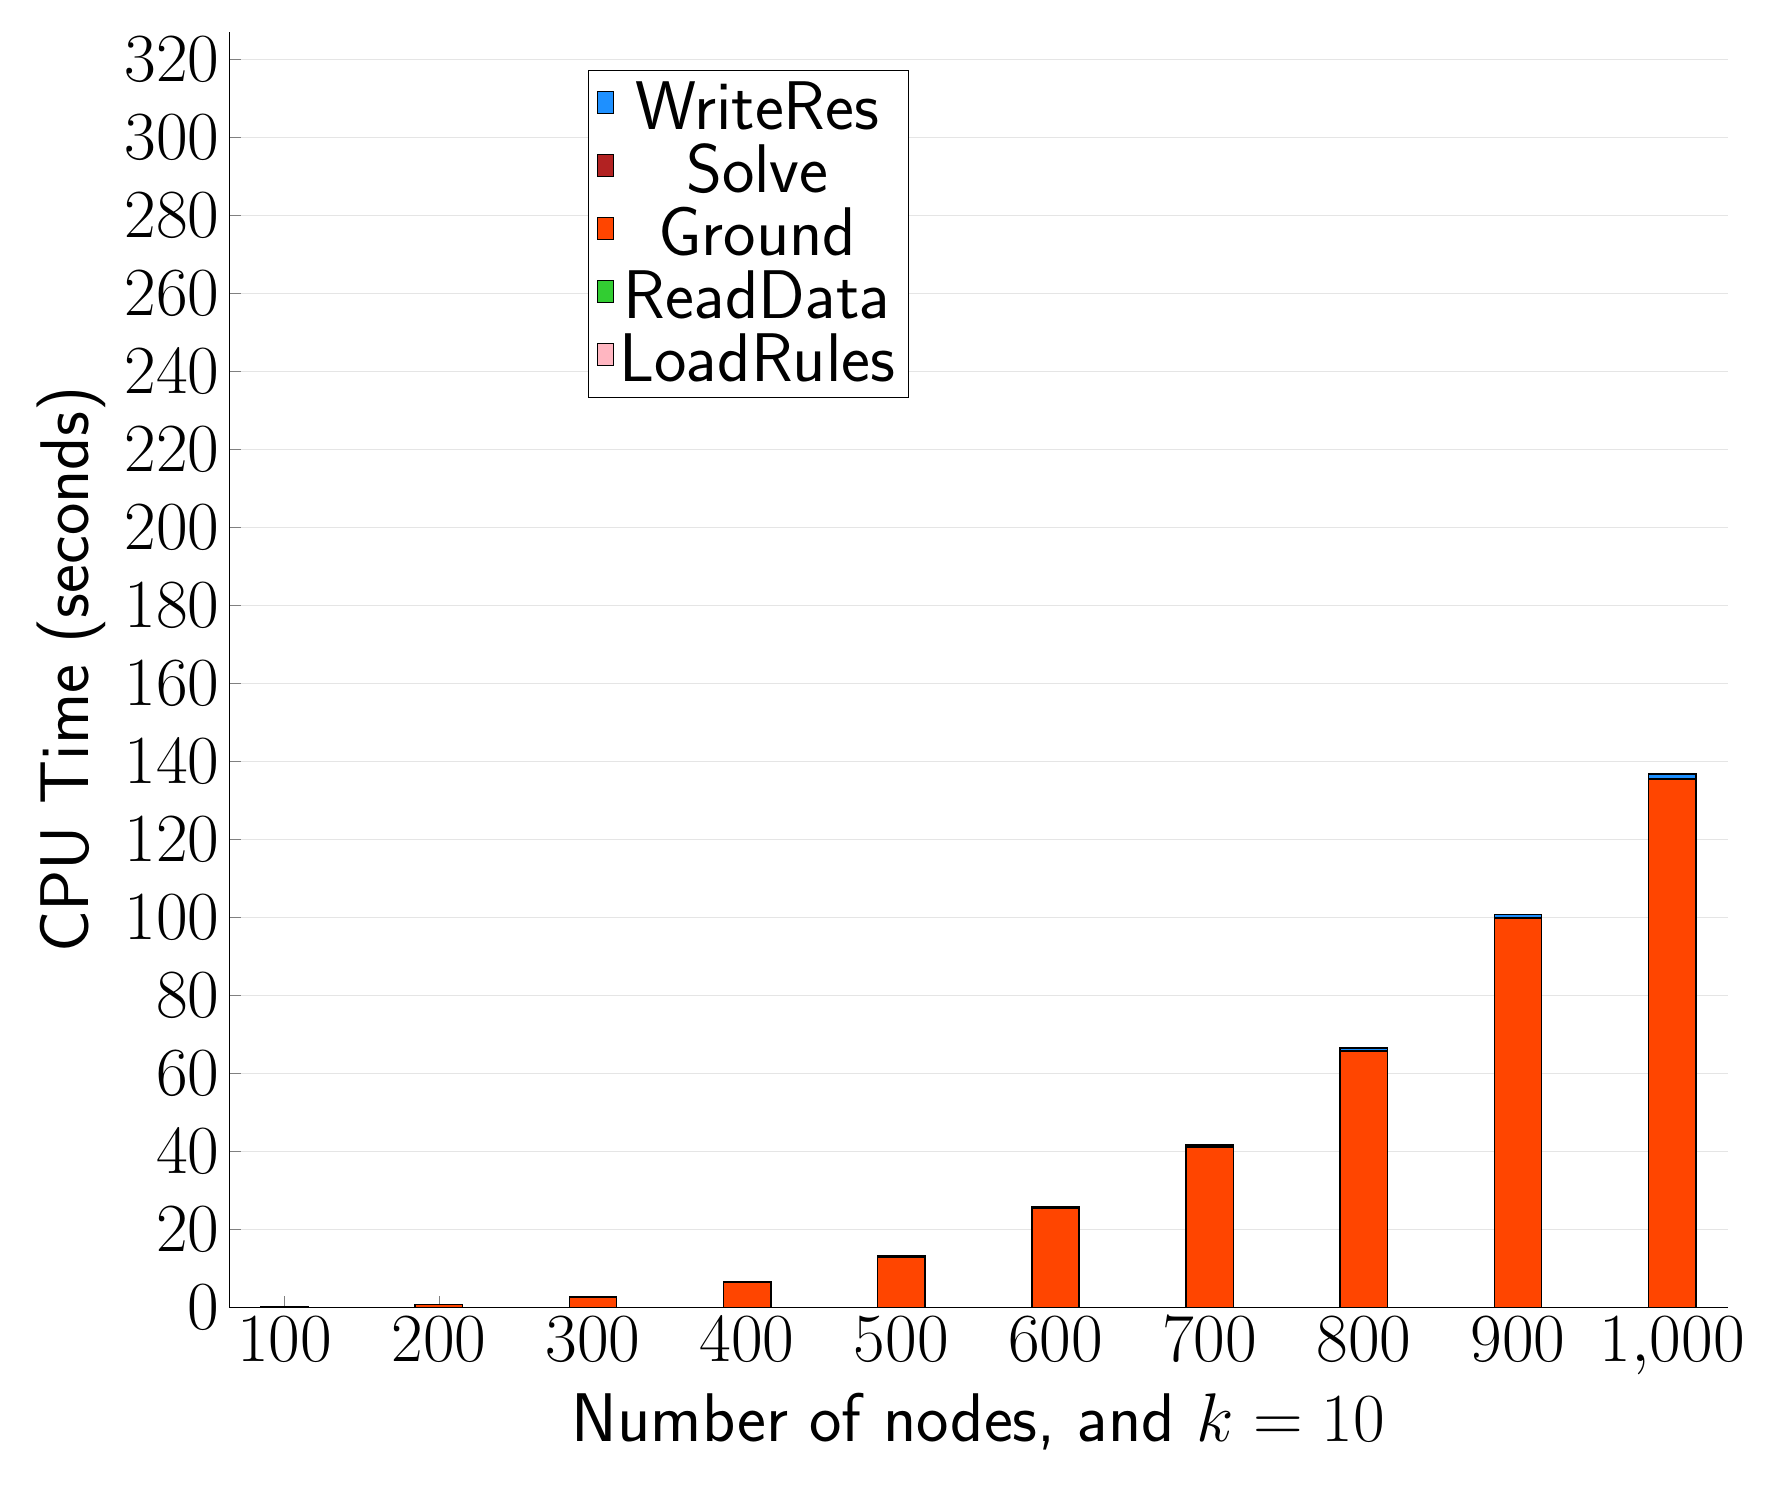
\begin{tikzpicture}
\begin{axis}[
   ybar stacked,
   width=1.7\textwidth,
   bar width=0.6cm,
   ymajorgrids, tick align=inside,
   major grid style={draw=gray!20},
   xtick=data,
   ymin=0, ymax=326.9108,
   axis x line*=bottom,
   axis y line*=left,
   enlarge x limits=0.04,
   legend style={
       at={(0.454, 0.97)},
       anchor=north east,
       legend columns=1,
       font=\Huge,
   },
   ylabel={CPU Time (seconds)},
   xlabel={Number of nodes, and $k=10$},
   label style={font=\Huge},
   tick label style={font=\Huge},
]
\addlegendimage{fill=DodgerBlue, draw=black, line width=0.2pt}
\addlegendentry{WriteRes}
\addlegendimage{fill=FireBrick, draw=black, line width=0.2pt}
\addlegendentry{Solve}
\addlegendimage{fill=OrangeRed, draw=black, line width=0.2pt}
\addlegendentry{Ground}
\addlegendimage{fill=LimeGreen, draw=black, line width=0.2pt}
\addlegendentry{ReadData}
\addlegendimage{fill=LightPink, draw=black, line width=0.2pt}
\addlegendentry{LoadRules}
\addplot +[fill=LightPink, draw=black, line width=0.55pt] coordinates {
(100, 0.0)
(200, 0.0)
(300, 0.0)
(400, 0.0)
(500, 0.0)
(600, 0.0)
(700, 0.0)
(800, 0.0)
(900, 0.0)
(1000, 0.0)
};
\addplot +[fill=LimeGreen, draw=black, line width=0.55pt] coordinates {
(100, 0.0)
(200, 0.0)
(300, 0.0)
(400, 0.010000000000000009)
(500, 0.010000000000000009)
(600, 0.010000000000000009)
(700, 0.01200000000000001)
(800, 0.018000000000000016)
(900, 0.020000000000000018)
(1000, 0.020000000000000018)
};
\addplot +[fill=OrangeRed, draw=black, line width=0.55pt] coordinates {
(100, 0.10000000000000005)
(200, 0.78)
(300, 2.694)
(400, 6.465999999999999)
(500, 12.978)
(600, 25.484)
(700, 41.068000000000005)
(800, 65.75999999999999)
(900, 99.78399999999999)
(1000, 135.46200000000002)
};
\addplot +[fill=FireBrick, draw=black, line width=0.55pt] coordinates {
(100, 0.0019999999999999905)
(200, 0.0)
(300, 0.009999999999999962)
(400, 0.008000000000000184)
(500, 0.011999999999999744)
(600, 0.020000000000000285)
(700, 0.029999999999999714)
(800, 0.03800000000000421)
(900, 0.0460000000000008)
(1000, 0.061999999999998404)
};
\addplot +[fill=DodgerBlue, draw=black, line width=0.55pt] coordinates {
(100, 0.007999999999999974)
(200, 0.050000000000000044)
(300, 0.10599999999999991)
(400, 0.18799999999999972)
(500, 0.3000000000000005)
(600, 0.4279999999999995)
(700, 0.5759999999999996)
(800, 0.7379999999999937)
(900, 0.9400000000000002)
(1000, 1.1480000000000055)
};
\end{axis}
\end{tikzpicture}

\end{document}
